\documentclass{standalone}

\usepackage{amsmath}
\usepackage{tikz}

\DeclareMathOperator*{\argmin}{argmin}

\usetikzlibrary{shapes, arrows.meta, positioning, backgrounds, angles, quotes, decorations.pathreplacing}

\tikzstyle{block} = [rectangle, minimum width=1cm, minimum height=1cm, text centered, draw=black, fill=white]
\tikzstyle{circ} = [circle, minimum width=.5cm, minimum height=.5cm, text centered, draw=black, fill=white]
\tikzstyle{arrow} = [->,>=stealth]
\tikzstyle{line} = [-]

\begin{document}
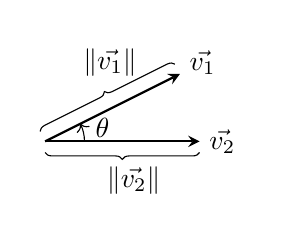
\begin{tikzpicture}[node distance=3cm, background rectangle/.style={fill=white}, show background rectangle]

    \coordinate (O) at (0, 0);
    \node (v1) at (2, 1) {$\vec{v_1}$};
    \node (v2) at (2.25, 0) {$\vec{v_2}$};

    \node at (.825, 1) {$\| \vec{v_1} \|$};
    \node at (1.125, -.5) {$\| \vec{v_2} \|$};

    \draw [line, decorate, decoration={brace, raise=4pt}] (O) -- (v1);
    \draw [arrow, thick] (O) -- (v1);
    \draw [line, decorate, decoration={brace, raise=4pt, mirror}] (O) -- (v2);
    \draw [arrow, thick] (O) -- (v2);

    \pic [draw, ->, "$\theta$", angle eccentricity=1.5] {angle = v2--O--v1};

\end{tikzpicture}
\end{document}